\part{Concepts théoriques}

\chapter[Monochr. et Polychr.]{Monochronique et Polychronique}

\paragraph{} D'après Edward Twitchell Hall, un anthropologue américain et
spécialiste de l'interculturalité, chaque culture a ses propres spécificités.
En effet, dans toutes les cultures il y a un mode de fonctionnement différent
lorsque nous évoquons les termes de délai de réalisation, de ponctualité, de
rythme ou de perception d'un évènement.

\paragraph{} Nous pouvons différencier deux cultures majeures différentes: le
temps monochronique et polychronique.

\section{Monochronique}

\paragraph{} Concernant les caractéristiques du temps monochronique, on peut
distinguer le fait que les personnes issues de cette culture font généralement
une chose à la fois. Par exemple au travail, un employé désirant qu'on l'aide
pour une tâche devra attendre que la personne à qui il demande finisse sa tâche
avant de l'aider. On peut remarquer cette différence de culture dans les
multinationales qui emploient plusieurs nationalités. Être sensibilisé à cette
différence de culture permet de mieux appréhender ses collègues et
éventuellement être tolérant envers eux.

\section{Polychronique}

\paragraph{} Au contraire, les personnes issues de la culture polychronique
auront tendance à se dispersé en faisant plusieurs tâches simultanément. En
effet, ils ressentent une charge affective qui les oblige à céder la priorité
aux relations personnelles plutôt que les relations d'affaires. Ils aiment
échanger de l'information pour apprendre à se connaitre.

\paragraph{} La culture monochronique prône le dicton ``le temps c'est de
l'argent'' et valorise donc la ponctualité et le respect des programmes
établis. L'objectif est d'être performant. Les personnes issues de la culture
monochronique sont contre toute interruption de leur travail qui briseraient
les actions. Concernant le domaine privé, leurs relations sont généralement
superficielles.

\chapter[Haut contexte, bas contexte]{Communication haut contexte et bas contexte}

\paragraph{} Les cultures à haut et bas contexte ont été définies par Edward T.
Hall en 1976 dans son livre Beyond Culture. Ces termes opposent les cultures
dans lesquelles les individus emploient un minimum de mots pour se faire
comprendre à celles où chacun s'exprime de manière explicite.

\section{Haut contexte}

\paragraph{} Dans une culture à haut contexte, une conversation au sein d'un
groupe n'est pas forcément compréhensible pour ceux qui n'en font pas partie,
car elle s'explique par l'histoire commune de ce groupe. En France, il est
courant de laisser planer le doute sur le sens d'une phrase, laissant à
l'interlocuteur le soin d'interpréter, ce qui peut troubler un Anglais, par
exemple (on prête à la culture anglaise un contexte plus bas). Ce dernier
verrait cela comme un manque de sincérité, alors qu'il s'agit plutôt pour le
Français d'une marque d'intimité. Le choix des mots devient très important,
puisque que chacun est chargé de sens : ils délivrent un message court et
efficace, mais qui à un mot près peut signifier le contraire.

\section{Bas contexte}

\paragraph{} À l'inverse, une culture à bas contexte accorde plus d'importance
à la clarté d'un message qu'à la portée de ses mots, et favorise les groupes
larges et ouverts à des groupes plus restreints mais plus intimes. C'est
pourquoi l'humour, dans une telle société, est plus facilement traduisible à
des étrangers, qu'ils soient issus d'une culture à haut ou bas contexte. Il est
toutefois plus difficile de marquer l'intimité par la conversation, car avoir
pour interlocuteur un proche n'impose pas d'édulcorer ses propos, mais plutôt
de faire preuve de franchise. Un Américain pourrait surprendre un Japonais par
la sincérité de ses propos, au risque de le vexer, car ces deux cultures ont
une vision différente de la préservation de la “face” : dans un bas contexte,
c'est en n'étant pas honnête avec l'autre (sur ses erreurs, ou ce qui l'attend)
qu'on l'humilie, tandis que dans un haut contexte, on met l'autre dans
l'embarras en ne lui laissant pas régler ses problèmes par lui-même.

\paragraph{} Bien qu'on ne puisse définir le contexte d'une société que
relativement à d'autres, et non comme absolument haut ou bas, ces concepts
permettent de mieux lire les échanges interculturels, afin de ne pas résumer
les membres d'une culture à haut contexte à leur orgueil, et ceux d'une culture
à bas contexte à leur manque de tact.


\chapter{Sphères publiques et privées}

\paragraph{} Le concept de sphère publique/sphère privée, ou vie privée/vie
publique est l'idée qu'une personne se situe soit dans une situation privée,
soit dans une situation publique, en fonction de l'endroit et des personnes aux
alentours. Cette théorie a été introduite en 1989 par Jürgen Habermas, connu
aussi pour la rationalité communicative. Jürgen Habermas décrit dans son livre
``La transformation structurelle de la sphère publique'' que la sphère
publique, et par extension la sphère privée, prends ses origines dans le
domaine de la bourgeoisie au 18\ieme{}siècle lors des salons mondains.

\section{Sphère publique}

\paragraph{} La sphère publique (en allemand: ``\textit{Öffentlichkeit}'') est
un espace de vie sociale en cohabitation où les personnes à l'intérieur de cet
espace parlent et agissent en respectant des règles et des lois sociales
tacites différentes en fonction des pays, régions, etc\ldots Ainsi les
opinions, les actions de la personne agissant dans la sphère publique ne
représente que la ``surface'' de la personne et ne correspond pas entièrement à
la personnalité et les volontés de la personne. Parmi les règles instaurées
implicitement on retrouve souvent :

\begin{itemize}
	\item L'abstention des sujets tabous.
	\item L'abstention d'actions déplacées
	\item L'abstention d'idées ou d'opinions trop ``extrêmes''.
\end{itemize}

\section{Sphère privée}

\paragraph{} La sphère privée, ou vie privée, est l'espace social, par
opposition à la sphère publique, où les personnes peuvent discuter et agir sans
prendre en considération les lois sociales et donc peuvent s'exprimer
totalement ou presque totalement en accord avec leurs opinions.

\chapter{4 dimensions culturelles}

\paragraph{} Geert Hofstede est un psychologue anthropologue hollandais qui a
étudié les interactions entre les différentes cultures, il est le référent dans
le management interculturel. Un jour IBM lui a demandé de prouver qu'il y avait
une forte culture d'entreprise chez eux. Pour cela, il a créé une théorie basée
sur 4 dimensions culturelles et en a tiré un questionnaire à choix multiple
auquel tous les employés ont répondu pour déterminer la force de leur culture
d'entreprise.

\paragraph{} Les quatre dimensions culturelles sont la distance hiérarchique,
l'individualisme, le contrôle d'incertitude et le niveau de
masculinité/féminité.

\section{Distance hiérarchique}

\paragraph{} La distance hiérarchique consiste au pouvoir fourni à une personne
face à ses subordonnés. En effet, dans un pays à forte distance hiérarchique,
les subordonnés ne doivent pas dire ce qu'ils pensent, ils doivent juste faire
ce qu'on leur dit. Par exemple, à la Cafeteria, lorsqu'il y a des étudiants en
train de faire la queue pour acheter un café, les professeurs ont tendances à
leur passer devant. Il s'agit ici d'une démonstration de forte hiérarchie :
même si les étudiants trouvent cette attitude immorale, ils se taisent et
prennent sur eux. Dans une culture à faible distance hiérarchique, il est
normal de contredire son supérieur si l'on n'est pas d'accord.

\section{Individualisme}

\paragraph{} L'individualisme consiste à valoriser la pensée personnelle. De ce
fait, dans une culture à fort individualisme, il est normal et valorisant de
dire ce qu'on pense et de réfléchir par soi-même. Au contraire, dans une
culture à fort collectivisme, la pensée de la collectivité est valorisée : la
collectivité est plus importante que l'individu. Il y a donc un lien entre
distance hiérarchique et individualisme. En effet, si l'on n'est pas d'accord
avec son supérieur on peut le contredire sans problème dans une culture
individualiste. Une culture individualiste a donc une faible distance
hiérarchique.

\paragraph{} Cependant, la France possède une forte distance hiérarchique bien
que ce soit une culture individualiste. En effet, les français peuvent
contredire leur chef s'ils ne sont pas d'accord mais le chef aura le dernier
mot.

\section[Incertitude]{Contrôle d'incertitude}

\paragraph{} Une culture à haut contrôle d'incertitude mettra tout en place
pour éviter les choses inattendues tandis qu'une culture à bas contrôle
d'incertitude sait très bien s'adapter face à l'inattendue puisqu'elle ne met
pas énormément de choses en place pour éviter celui-ci.  Ainsi, une culture à
haut contrôle d'incertitude sera normative : beaucoup de normes seront
inventées pour éviter de se trouver face à un inconnu. Une culture à bas
contrôle d'incertitude sera plus pragmatique : l'inattendu fait partie de la
vie, c'est ce qui la rend intéressante, il n'est donc pas nécessaire de
l'éviter à tout prix.

\section{Masculinité/Féminité}

\paragraph{} Le niveau de masculinité d'une culture dépend des valeurs
valorisées par cette culture. Une culture masculine valorise le succès et la
réussite tandis qu'une culture féminine valorise la modestie et la compassion
pour les plus pauvres et ceux qui ont moins bien réussi dans leur vie. Par
exemple, le Japon et l'Allemagne sont des cultures à fort niveau de masculinité
tandis que la France et la Suède sont des cultures à fort niveau de féminité.

\section{Test des 4 dimensions}

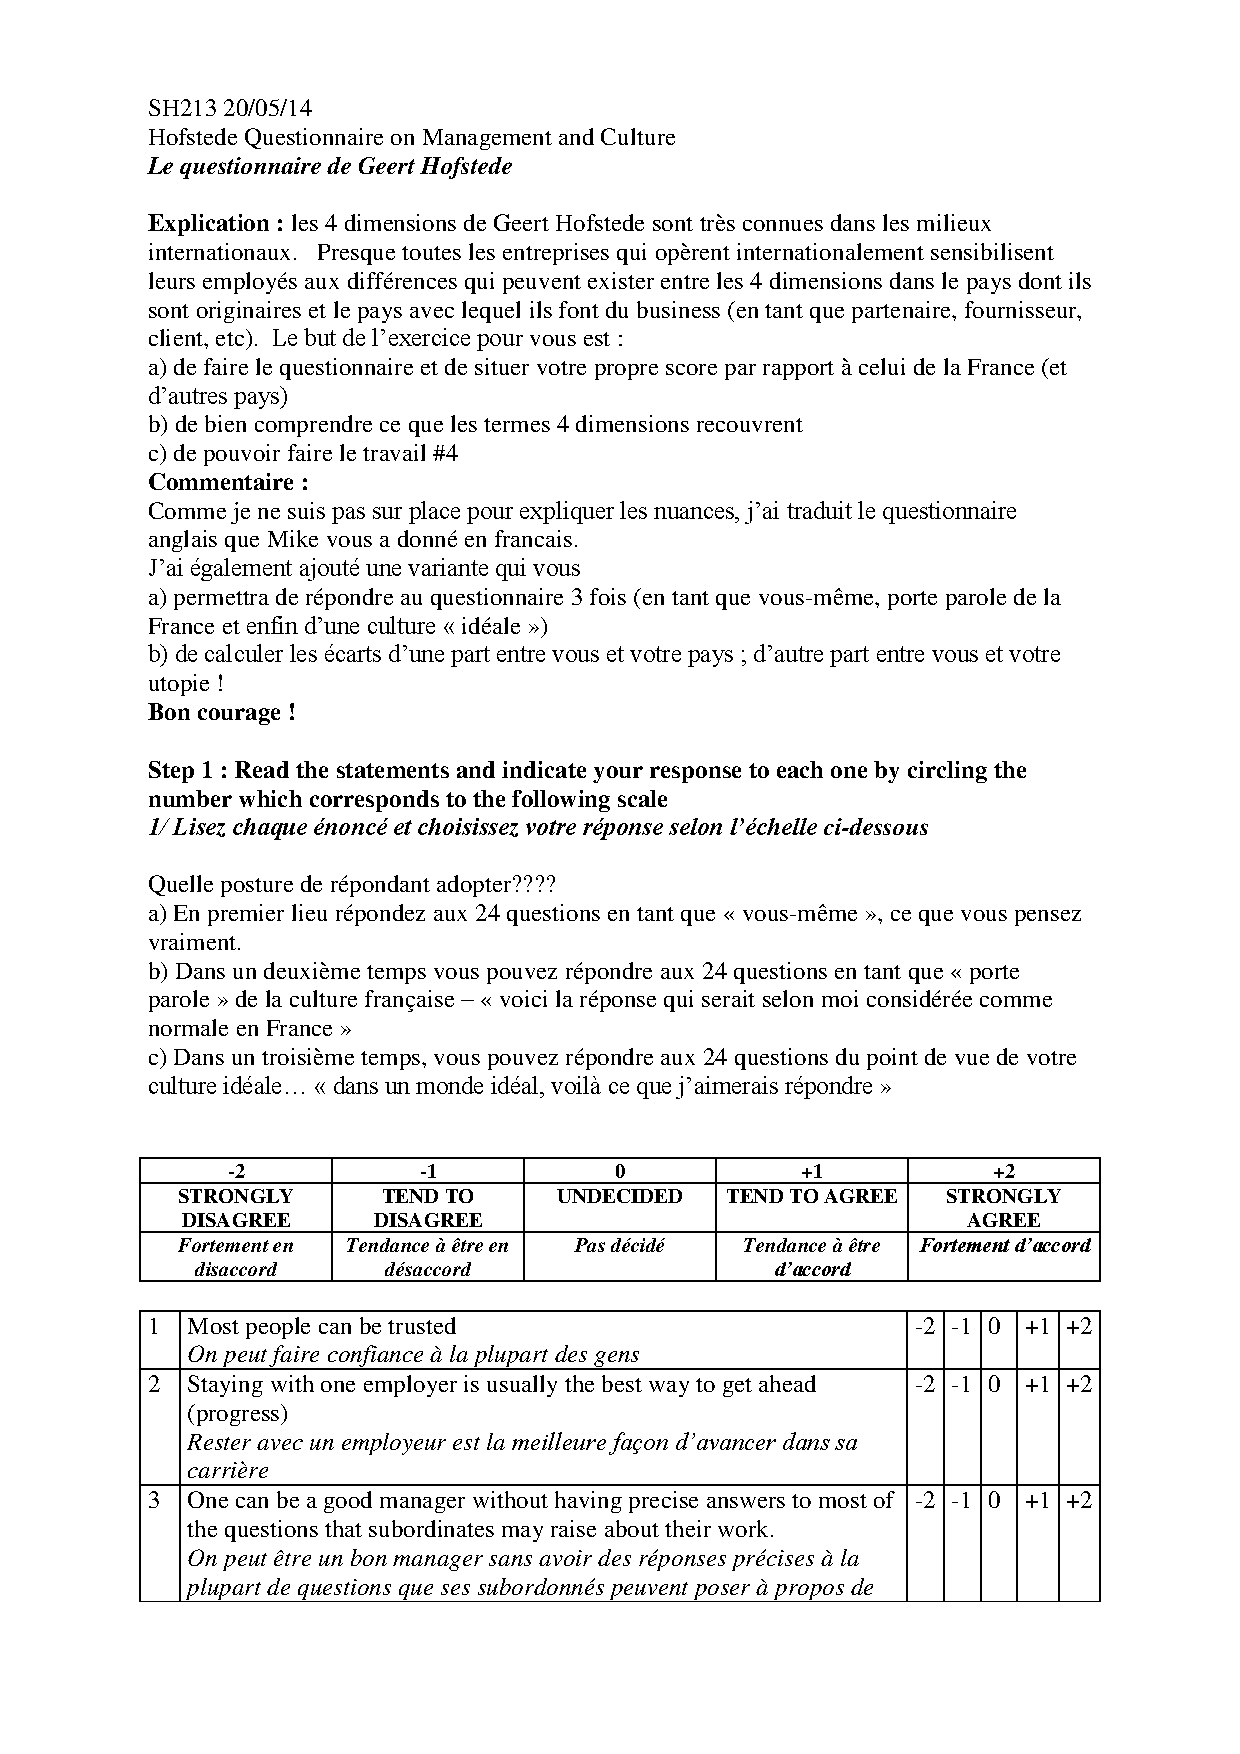
\includepdf[pages = {1-9}]{hofstedequestfrancais.pdf}
